\documentclass{standalone}
\usepackage{tikz}
\usetikzlibrary{automata,positioning}

\begin{document}
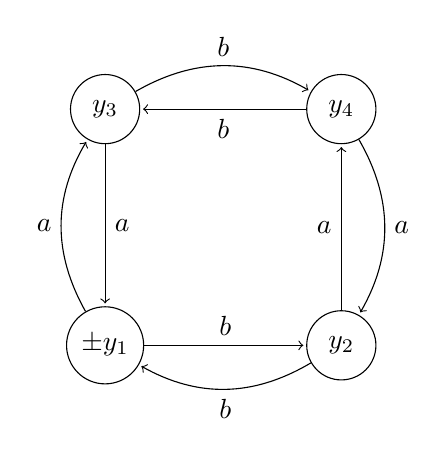
\begin{tikzpicture}[shorten >=1pt,node distance=3cm,on grid,auto]
  \node[state] (q1) at (0,0) {$\pm y_1$};
  \node[state] (q2) at (3,0) {$y_2$};
  \node[state] (q3) at (3,3) {$y_4$};
  \node[state] (q4) at (0,3) {$y_3$};

  \path[->]
    (q1) edge [bend left] node {$a$} (q4)
    (q1) edge node {$b$} (q2)
    (q2) edge node {$a$} (q3)
    (q2) edge [bend left] node {$b$} (q1)
    (q3) edge [bend left] node {$a$} (q2)
    (q3) edge node {$b$} (q4)
    (q4) edge node {$a$} (q1)
    (q4) edge [bend left] node {$b$} (q3);
\end{tikzpicture}
\end{document}